\documentclass{article}

\usepackage[T1]{fontenc}
\usepackage[utf8]{inputenc}
\usepackage{mdwlist} % To have compact lists
\usepackage{hyperref} % To have links to URLs
\usepackage{float} % To force images to the right place
\usepackage{listings} % To display source code
\usepackage{csquotes} % To display blockquotes
\usepackage{caption}
\usepackage{subcaption}


% To include images
\usepackage{graphicx} 
\graphicspath{ {images/} } % location of images

% To adjust image position
\usepackage[export]{adjustbox}

% To add hyperlink
\usepackage{hyperref}

% Disables automatic indents globally
%\setlength{\parindent}{0pt}

% Set link color to blue
%\hypersetup{
%    colorlinks=true,
%    linkcolor=blue,
%    filecolor=blue,      
%    urlcolor=blue,
%    citecolor=blue
%}


\begin{document}

%================================== Header Begins =============================
\begin{center}
	{\LARGE \textbf{Evaluation Report}} \\
	\vspace{0.5em}
	\textsl{Team $\lambda$ Lovelace}
\end{center}

\vspace{0.5em}

\begin{center}
	29th July 2016 \\
	COMP47250, Team Software Project 2016 \\ 
	University College Dublin, Ireland \\
\end{center}

\vspace{0.5em}
%================================== Header Ends ===============================



\noindent This is an evaluation report for the team $\lambda$ Lovelace, summer 2016. The module formally started 2016.05.16 and will end in a final code \& report submission on 2016.08.19. This document was submitted eleven weeks after the start of the project.


%==============================================================================
\section{Hypothesis}
% 500 words
%
% Explain the questions you are asking in your experiment and why they are 
% important. Also provide an overview of some interesting, important, and 
% relevant existing work in relation to evaluating such hypothesis (e.g., how 
% is this hypothesis typically evaluated, do previous evaluations, if any, have 
% any flaws?). For existing work provide appropriate citations and screenshots.
%
For this experiment, team $\lambda$ Lovelace is asking the question:

\begin{center}
    ``\textit{Is $\lambda$ Lovelace's personalised tweet feed more interesting to the user than the default chronologically ordered tweet feed from Twitter?}''
\end{center}

Team $\lambda$ Lovelace's goal is to show that it can be preferable for the user to have short-term recommendations. We believe that the hypothesis is an important question to ask, due to both the ubiquitous nature of Twitter and the powerful effect of recommender systems. Entire businesses revolve around the strength of their recommender systems, so team $\lambda$ Lovelace attempts to marry the popular platform of Twitter with the personalisation of recommendation.

\subsection{Related Work}
In the course of the creation of this experiment, team $\lambda$ Lovelace identified three particularly interesting examples of similar experiments, relevant to the experiment to be performed. In \textit{Towards a Followee Recommender System for Information Seeking Users in Twitter} \cite{paper1}, the authors perform a very similar experiment to team $\lambda$ Lovelace, with the exception of the data collection, and found success. While both teams take a quantitative approach to their experiments, Marcelo G. Armentano et. al required users to perform these tests on a desktop computer. This approach is much easier to implement than team $\lambda$ Lovelace's use of multiple mobile devices. 

This paper also describes how the authors requested that users create new accounts with fresh data. This approach, although not applicable to the $\lambda$ Lovelace system, would have been more convenient for testing purposes if the $\lambda$ Lovelace system did not require power users. "Power users" being regular Twitter users that generally follow hundreds of accounts and have hundreds of tweets, retweets and likes. Overall, this is a very similar testing approach to team $\lambda$ Lovelace, as the system tested also provided somewhat similar functionality, that of twitter recommendations.
\\\\
In \textit{Recommending Twitter Users to Follow Using Content and
Collaborative Filtering Approaches} \cite{paper2}, the authors perform two forms of testing, a preliminary offline experiment and a live user trial experiment. This allowed the authors to make initial assumptions on their project before beginning the live user trials, which would be more difficult to organise and take more effort. It was a much "safer" choice to hold a preliminary experiment before the main experiment.
\\\\
In \textit{Using Twitter to Recommend Real-Time Topical News} \cite{paper3}, the authors tackle a similar topic to \textit{Towards a Followee Recommender System for Information Seeking Users in Twitter}, but perform user testing over a period of five days. This allowed the authors to gain data outside of a testing environment, although this would be much more difficult to enforce upon participants.

Team $\lambda$ Lovelace incorporates an aspect of this open style of testing by allowing participants to come and test over a period of several hours, rather than a scheduled approach. This paper also revealed a discrepancy between what the participants say they prefer, and what they actually prefer when dealing with content recommended from twitter or content that is followed by their twitter friends. This influenced team $\lambda$ Lovelace to use more objective methods when testing.


% the only similar evaluation I can think of to ours is how Twitter itself 
% evaluated their recommendation. If I recall correctly Twitter measured 
% their success by increase in engagement, which is good for their wallet but 
% we feel it may not achieve our goal: to show interesting tweets to users.
% Basically Twitter's goal is to have users engage a lot. Our goal is to provide 
% a recommendation system for lurkers AND active users.

%Marc: The question we are asking is whether or not a recommender system can provide greater value to a twitter user than simply having tweets come at them in real time. Existing work could possibly be taken from some earlier work for documents we did for this module, such as the work for flipboard, etc. Flaws should definitely be mentioned here, like how some people will give us innaccurate  feedback jus because they want some reward we're giving them, etc. And biased family members/friends not giving back good data.

%==============================================================================
\section{Experimental Method}
\subsection{Overview}
% 250 words
%
% How will you run your experiment? What will the experimental conditions be? 
% What is your overall experimental design? What are the baselines you compare 
% against and the evaluation metrics?
%

%Marc: We may just want to mention the evaluation app for this section. Based on how the task is phrased, it seems to be hinting at a once-off experiment, rather than the long-term effects that likes/dislikes will have on the recommender system. Might be worth emailing about this to clarify.
%For this experiment, team $\lambda$ Lovelace has prepared an evaluation-specific version of the $\lambda$ Lovelace application, which will be used in this experiment. This app will allow participants to rate batches of tweets from their original timeline, and the timeline created by $\lambda$ Lovelace's recommender system. Participants will be presented with each of these feeds, then the evaluation app will allow them to rate one as superior to the other.
For this experiment, team $\lambda$ Lovelace has prepared an evaluation-specific version of the $\lambda$ Lovelace application, which will be used in this experiment. This app will allow participants to rate individual tweets if they are interesting to them: thumbs up, neutral, thumbs down.

\begin{figure}[H]
    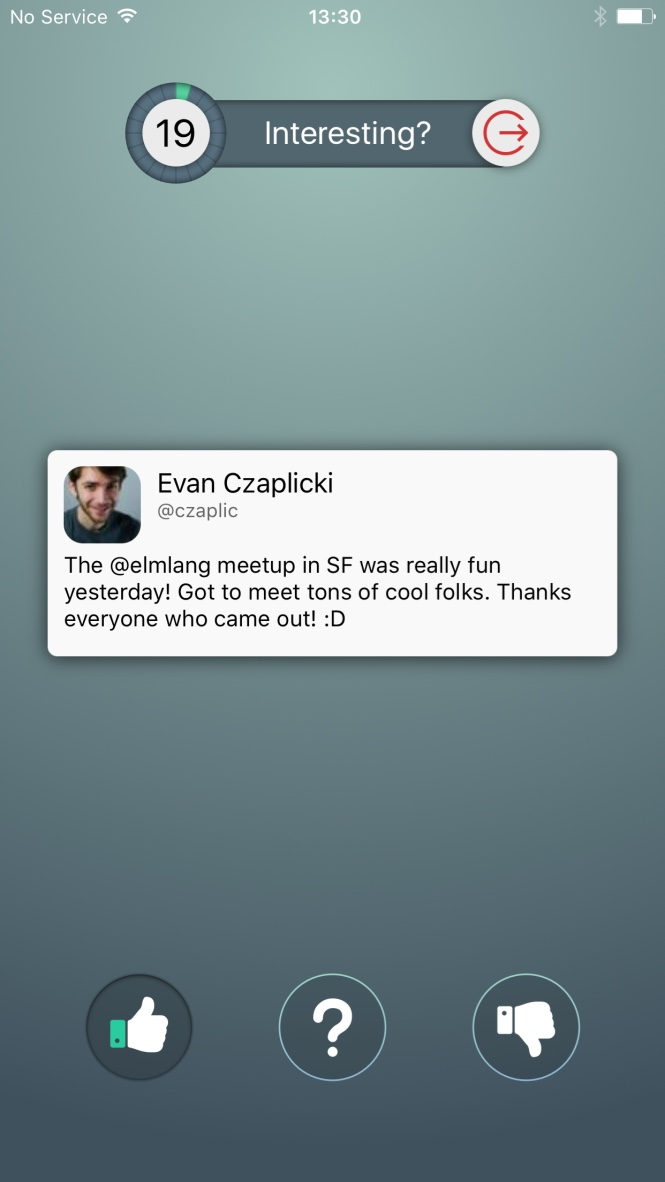
\includegraphics[width=0.4\textwidth, center]{eval1}
    \caption{Screenshot from the evaluation iOS app}
\end{figure}

Each evaluation run has the user rate a batch of twenty tweets at a time. An evaluation session can consist of multiple runs, as many as the evaluator has patience for. However the plan is that each evaluation session should take about fifteen minutes to complete. Each batch of twenty tweets is sourced from two Twitter feeds. The top ten from the default chronologically ordered Twitter feed\footnote{in the Twitter API this is referred to as the \textit{homeline}} and the top ten from $\lambda$ Lovelace's feed. The evaluator will not know from which feed the tweet came.

\begin{figure}[H]
    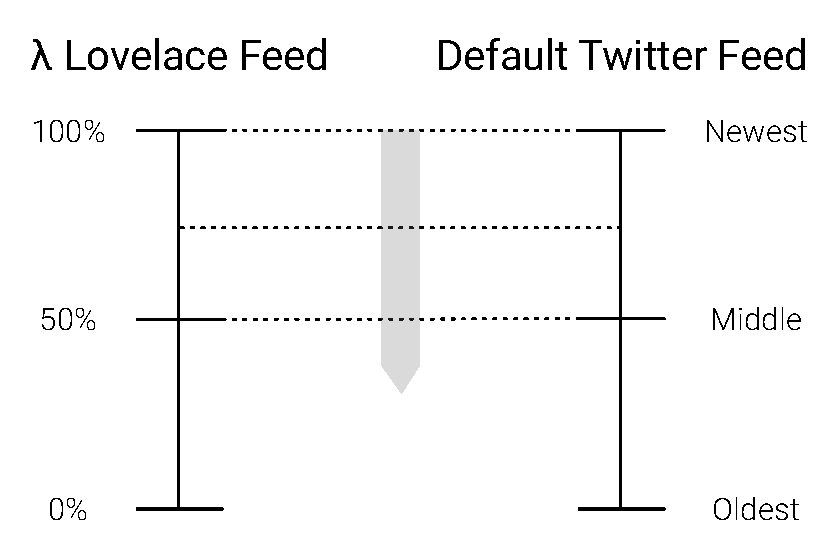
\includegraphics[width=0.6\textwidth, center]{evaluations_1}
\end{figure}

\newpage

From the data gained from this experiment, team $\lambda$ Lovelace hopes to draw conclusions on the quality of $\lambda$ Lovelace's recommended tweets. For these purposes, participants will have to log into the $\lambda$ Lovelace app with their personal Twitter account.
\\\\
Participating subjects will be largely drawn from college-aged students who are familiar with Twitter, allowing team $\lambda$ Lovelace closer access to the power users that this system is aimed at. This experiment will take place in B0.02 of the Computer Science and Informatics building on University College Dublins Belfield campus, allowing for a short travelling distance, ample room for potentially large numbers of participants and an organised environment.
\\\\
Metrics used for this experiment will be drawn from the results of the evaluation app. These metrics reflect sentiment for batches of tweets from both the original timeline and $\lambda$ Lovelace's recommender system. Tweets can either have positive(liked), negative(disliked) or neutral(neither) sentiment. The score of both the recommender system and the original timeline is tallied up to discern the more well-received system.

\subsection{Data Collection}
% 250 words
%
% What data will you collect during the experiment about participants’ performance 
% and why? Will there be a mix between subjective (qualitative) and objective 
% (quantitative) measurements? How does the data you will collect relate directly 
% to your experimental hypothesis?
%
%Marc: We probably want to get the test users to give the app a few "runs" so that they like/dislike with the evaluation app. We should prepare a questionaire for them too with an open-ended comments section. The questionaire should be given a second-look by family members/friends however, so we know that we aren't asking less fruitful/useful questions.

Data collected by the participants will be of a quantitative nature, where team $\lambda$ Lovelace can view the results of each evaluation and infer preference for either the official Twitter timeline, or the $\lambda$ Lovelace feed. The metrics used will be numerical, with each like adding to the "score" of either the offical Twitter timeline or the $\lambda$ Lovelace evaluation app. Team $\lambda$ Lovelace intends to capture the users interests with the recommendations provided, so should be scored higher than the default Twitter timeline.
\\\\
From this data, team $\lambda$ Lovelace will be able to compare $\lambda$ Lovelace's recommendations with Twitter's chronological tweet feed. Finally, from this comparison it can be conclusively determined which form of Twitter feed provides more value to the user, answering the question raised in this papers hypothesis. Qualitative data will not play a part in this experiment, as team $\lambda$ Lovelace does not have the time or resources to filter good qualitative data from unintentionally dishonest data from the participants. This decision allows team $\lambda$ Lovelace to focus more on the evaluation app as the main strength of the experiment, rather than requesting participants to perform several different forms of testing, which could tire out or otherwise bore participants, which could in turn affect the resulting dataset.
\\\\
The collected data will be stored in RethinkDB\footnote{a document database where each "row" is a JSON object} so that it is accessible in the same manner as both the live and test tweet data sets. 

\begin{samepage}
\noindent Here is a pseudo example JSON data submitted for an evaluation run:
\begin{verbatim}
{
    "id": "4c1c9819-df34-4803-9678-fbeab7641c02",
    "time": 1469724613038,
    
    "user_info": {
        "screen_name":  "lambda_lovelace",
        "tweets_liked": 1337,
        "tweets_of_me": 824,
        "users_following": 432
    },

    // Aggregate tally of results for this evaluation run
    "counts": {
        "originalDislike": 3,
        "originalLike": 4,
        "originalNeither": 3,
        "recommendDislike": 2,
        "recommendNeither": 4,
        "recommendLike": 4
    },
    
    "result": [
        {
            "source": "original", // Twitters default feed
            "tweetId": "758705114785910785",
            "userOption": "like", // User liked the tweet
            "userScreenName": "@smarimc"
        },
        
        ... // 19 other tweets
    ]
}
\end{verbatim}
\end{samepage}

\subsection{Selected Subjects}
% 250 words
%
% Who will you use as subjects in your experiment. Why are these a representative 
% sample? How will you source these subjects?
%
Subjects for the pilot evaluations will be chosen from amongst team $\lambda$ Lovelace's family, friends and acquaintances. This will not be the main experiment for this project, due to the bias present in this group and the relative lack of good-quality participants.
\\\\
This preliminary experiment will serve as a filter for the main experiment. In this first experiment it is hoped that outsider perspectives will reveal issues with the software that team $\lambda$ Lovelace did not initially anticipate. As there is a limited amount of time left for this project, we are constrained in how many of the main experiments we can hold. As the results of this experiment may reveal untrue assumptions about this entire project, it is vital that any errors are revealed before the main experiment, as fundamental errors could result in useless data. It may be possible to hold another main experiment if the first attempt at one is botched through fundamental error, but due to a lack of time, it would be unwise to assume so. 
\\\\
The main experiment will consist of college-level students, sourced from University College Dublin who are active Twitter users. These will be obtained through flyers distributed throughout the University grounds that advertise the experiment on a given date. It will be made clear that the user must be an active Twitter user that often likes/retweets/tweets on the platform. Team $\lambda$ Lovelace will also check the participants personal homeline to prevent dishonest participants from attending, where they simply create a twitter account and create multiple fake tweets/retweets to give the impression of a genuine regular Twitter user.
\\\\
If possible, the Computer Science: Negotiated Learning and Conversion MSc courses will be used for the main experiment. These may be the easiest group of students to access, the "low-hanging fruit" that can provide us with valuable data.

\subsection{Data Analysis}
% 250 words
%
% How will you analyse the data you collect during the experiment? How will this 
% analysis answer the question you originally proposed?
%
Team $\lambda$ Lovelace brainstormed upon this several times and ultimately decided to take the simplest approach. That is, team $\lambda$ Lovelace will compare the $\lambda$ Lovelace version of the Twitter feed to the default home timeline. The version that gains more "likes" in the evaluation app will be judged the better version with concerns to relevancy. Thus answering this papers original question of "Is $\lambda$ Lovelace's personalised tweet feed more interesting than the default chronologically ordered tweet feed from Twitter?" with hard data.
\\\\
It is not left to the participant to critically think about whether one whole offering (The $\lambda$ Lovelace app or the official Twitter website) is better. Rather, this form of experimentation requests only the most basic of preference (This tweet or that tweet) and allows team $\lambda$ Lovelace to analyse the results. Requesting more complex tasks from participants can lead to pitfalls in experimentation, as seen in \textit{Using Twitter to Recommend Real-Time Topical News} \cite{paper3}, where participants voiced an opinion that later revealed to be entirely untrue.
\\\\
This form of analysis, due to its numerical data, will also allow team $\lambda$ Lovelace to graph the resulting dataset for comprehension purposes. This data can be used in a variety of methods to extract information, but is limited in how much it allows the user to express. For example the user cannot, with this method, explain why they prefer one tweet over another. The user cannot, likewise, explain why they dislike another tweet over another. However extracting such information would be a time-consuming task, beyond the resources at team $\lambda$ Lovelace's disposal at this time of writing.

\begin{figure}[H]
    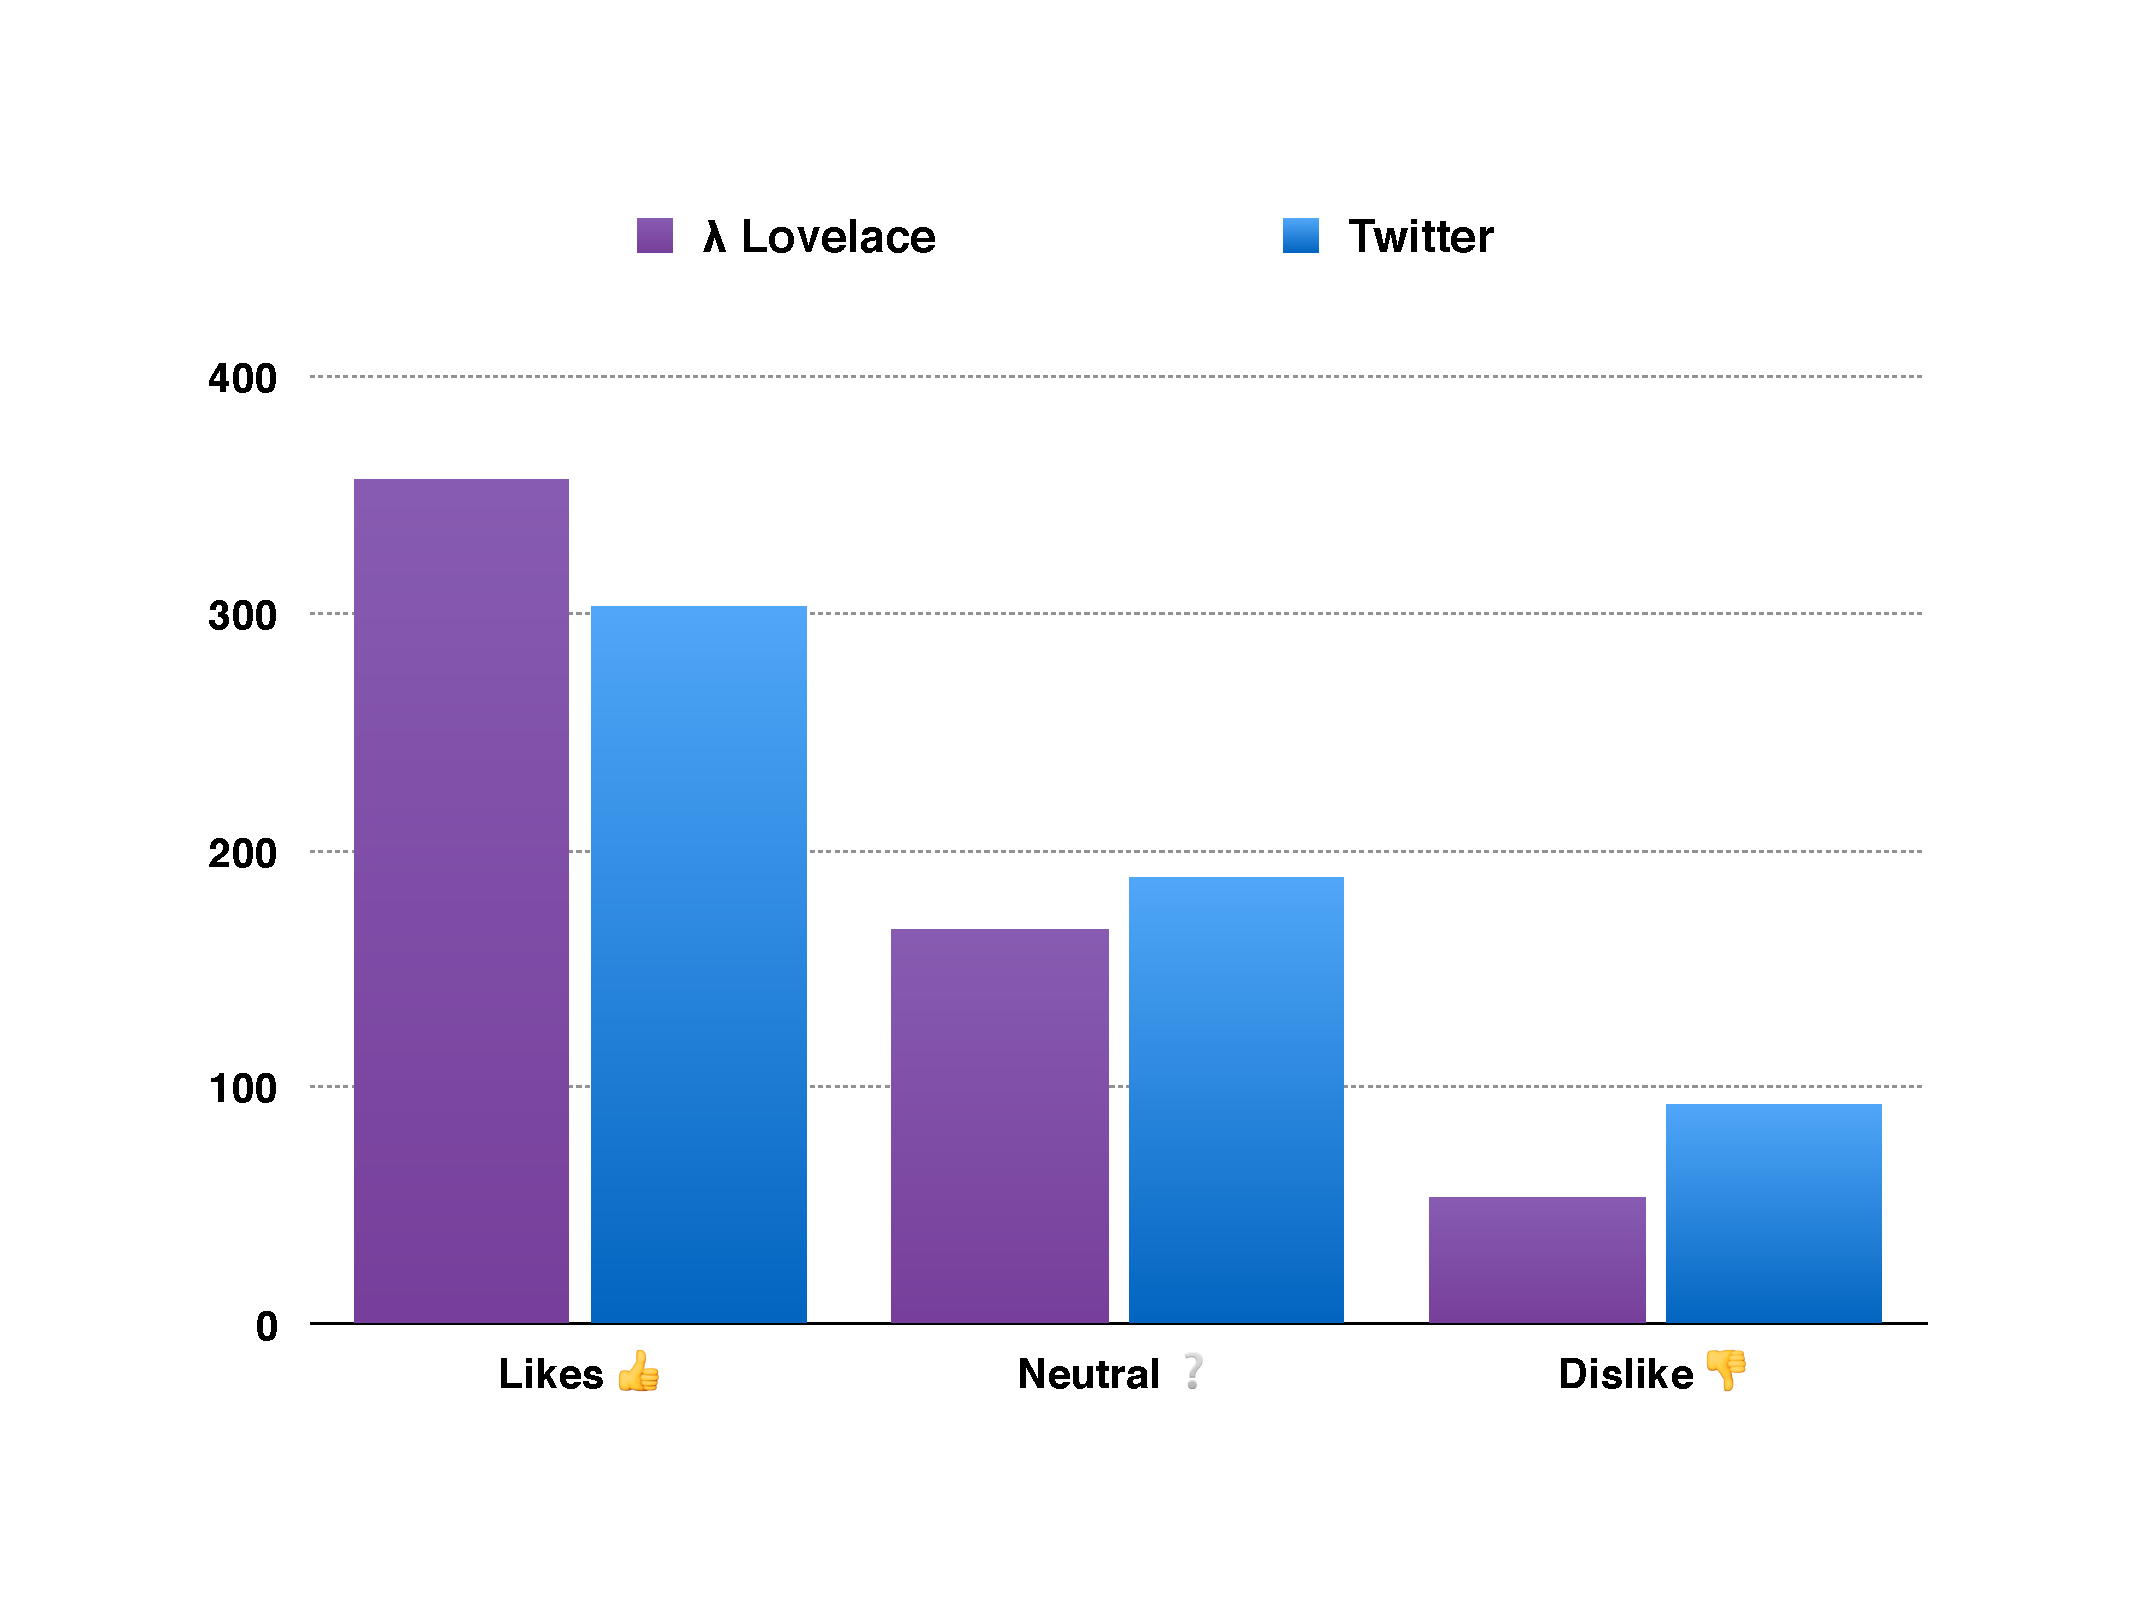
\includegraphics[width=1\textwidth, center]{sample_graph}
    \caption{Example how the data will be analysed. Please note the numbers are fake as the true evaluation runs have not yet taken place.}
\end{figure}


\subsection{Practical Setup}
% 250 words
%
% In practical terms how will you run your experiment? Will it be online or 
% offline? What instructions will participants be given? What type of 
% room/environment will the experiment be in? Will questions/surveys be displayed 
% on-screen or on printed paper?
%
% 292 words currently
The experiment will be run within room B0.02 in the Computer Science building at University College Dublin. The experiment will run for the majority of an afternoon during the month of August. The purpose of this setup is to allow participants ease of access for the duration of the experiment. We believe that fewer barriers for participation will yield higher turnout, so allowing participants to show up at their convenience will prevent the discouragement that presents itself in strict scheduling for an experiment. 
\\\\
The choice of room is both a convenient choice and an appropriate one. The rooms in the ground floor of the Computer Science and Informatics building have been used before for University College Dublin's end-of-semester exams. So these rooms have proven capable of holding large numbers of students and providing a sterile and organised environment for the purpose of testing, as they have been used for examination-test purposes before. 
\\\\
The app will be ready to run on four of team $\lambda$ Lovelace's iPhone devices, so that there is no need for the participants to install the software. This should speed up the experimentation process, and further remove the barriers to entry for the user. The only thing the user has to do is sign in with their own Twitter credentials.
\\\\
In addition to running the experiment in person, team $\lambda$ Lovelace has published the evaluation app via the beta mobile app distribution platform HockeyApp \cite{hockeyapp}. Team $\lambda$ Lovelace has had success so far but the setup process is a bit time-consuming for the potential evaluator. It's not intended as the primary source of participants but more of a backup if physical turnout is low.
\\\\
There will be no questions asked, rather the participant will use the evaluation version of the $\lambda$ Lovelace app. They will be asked to perform the evaluation process for as long as they are willing. The evaluator is presented with twenty tweets at a time and results from each batch is uploaded. An evaluation session will take approximately fifteen minutes to complete. The results of the participants efforts will be stored and conclusions will be drawn from this information.

%==============================================================================
\section{Conclusion}
% 250 words
%
% What can you conclude after running this evaluation study (have you learned 
% anything useful about the quality of your solution)? What could be done better 
% in a future evaluation study (e.g., would you ask different questions or use 
% different evaluation metrics)?
%
Upon completion of this experiment, team $\lambda$ Lovelace should be capable of concretely answering the original question posed in the hypothesis. If given more time to organise and gather resources, it may have been possible to conduct several higher quality tests with more participants. With enough time, it would have been possible to test for qualitative data, which could possibly reveal more information about the participants reasoning behind liking or disliking a tweet, or even overall feedback about the $\lambda$ Lovelace app itself.
\\\\
Given more time, an ideal experiment setting would involve allowing the participants to use the $\lambda$ Lovelace app over the course of several days. The $\lambda$ Lovelace app could have temporarily replaced the participants use of the official Twitter website and the users could respond at the end of a week with their level of satisfaction with the app. Further testing could involve requesting participants to give their level of satisfaction on a daily basis, with team $\lambda$ Lovelace tweaking several of the attributes of the recommender system (Number of terms in the term frequency document, values given to hashtags and liked/disliked tweets, etc) and observing the effect on participants satisfaction levels. This form of testing is not without its disadvantages, as participants can give inaccurate feedback when critical thinking is involved. However this could be circumvented, resources permitting.
\\\\
Overall, this experiment will be useful for the purposes of evaluating the $\lambda$ Lovelace application. However like most endeavours, there will always be space for improvement. 


\newpage


%==============================================================================
\section{Appenix}
% This appendix contains information for a historical perspective such as what Twitter is and who the students and professors are. 

\subsection*{Students \& Professors}
The group project is the third and final semester of the Negotiated Learning MSc in Computer Science at University College Dublin. The students and professors involved are:
        
\begin{samepage}
\begin{center}
\begin{minipage}[t]{.4\textwidth}
	\textbf{Students}:
		\begin{itemize*}
			\item Xinqi Li
			\item Marc Laffan
			\item Junyang Ma
			\item Jón Rúnar Helgason
			\item Eazhilarasi Manivannan
		\end{itemize*}
\end{minipage}
~
\begin{minipage}[t]{.4\textwidth}
	\textbf{Module co-ordinators}:
	\begin{itemize*}
		\item Dr. Georgiana Ifrim
		\item Dr. Brian Mac Namee
		\item Dr. Derek Greene
	\end{itemize*}
\end{minipage}
\end{center}
\end{samepage}

\vspace{2em}


%==============================================================================
%                               References
%==============================================================================
\begin{thebibliography}{9} 

\bibitem {paper1}
    Marcelo G. Armentano and Daniela Godoy and Analía Am. Towards a Followee Recommender System for Information Seeking Users in Twitter.  In \textit{Proceedings of the Workshop on Semantic Adaptive Social Web (SASWeb 2011)}. CEUR Workshop Proceedings, volume 730, pages 27–38, 2011.
    
\bibitem {paper2}
    J. Hannon, M. Bennett, and B. Smyth. Recommending twitter users to follow using content and collaborative filtering approaches. In \textit{Proceedings of the fourth ACM conference on Recommender systems}, pages 199–206. ACM, 2010.
    
\bibitem {paper3}
    O. Phelan, K. McCarthy, and B. Smyth. Using Twitter to recommend real-time topical news. In \textit{Proceedings of the third ACM Conference on Recommender Systems}, pages 385–388. ACM, 2009.
    
\bibitem {hockeyapp}
    HockeyApp, \url{https://hockeyapp.net/}
	
\end{thebibliography}


\newpage

\end{document}